% Tik output from JumanG
\documentclass[class=minimal,border=0pt]{article}
\usepackage{tikz}
\pagestyle{empty}
\usepackage{verbatim}
\begin{document}
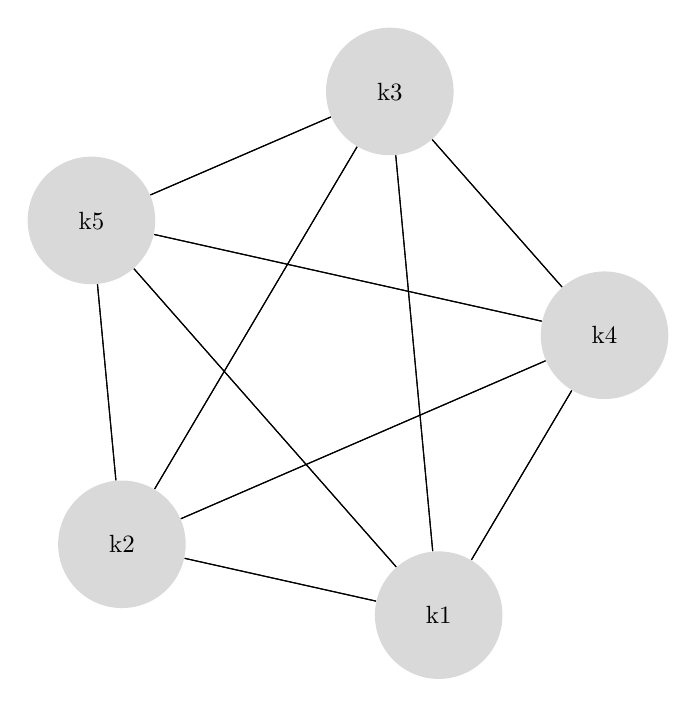
\begin{tikzpicture}[scale=0.90, transform shape]
	\tikzstyle{every node} = [circle, fill=gray!30, minimum size = 1.8cm]
	\node (k3) at (0.72, 3.87) {k3};
	\node (k2) at (-3.06, -2.52) {k2};
	\node (k1) at (1.41, -3.52) {k1};
	\node (k5) at (-3.49, 2.05) {k5};
	\node (k4) at (3.75, 0.43) {k4};
	\draw [-] (k3)--(k1);
	\draw [-] (k3)--(k2);
	\draw [-] (k3)--(k4);
	\draw [-] (k3)--(k5);
	\draw [-] (k2)--(k1);
	\draw [-] (k2)--(k3);
	\draw [-] (k2)--(k4);
	\draw [-] (k2)--(k5);
	\draw [-] (k1)--(k2);
	\draw [-] (k1)--(k3);
	\draw [-] (k1)--(k4);
	\draw [-] (k1)--(k5);
	\draw [-] (k5)--(k1);
	\draw [-] (k5)--(k2);
	\draw [-] (k5)--(k3);
	\draw [-] (k5)--(k4);
	\draw [-] (k4)--(k1);
	\draw [-] (k4)--(k2);
	\draw [-] (k4)--(k3);
	\draw [-] (k4)--(k5);
\end{tikzpicture}
\end{document}
